\documentclass{beamer}
\usepackage[utf8]{inputenc}
\usepackage{xmpmulti}
\usepackage{subfigure}
\usepackage[small]{caption}
%\usetheme{JuanLesPins}
\usetheme{Padova}

%STRUTTURA:
%DTN
%M2MShare
%ONE
%modelli movimento: WDM

          
\author{Daniele Bonaldo}
\title{Performance Evaluation with Realistic Mobility of a File Sharing DTN Protocol}
\institute{UNIVERSITÀ DEGLI STUDI DI PADOVA\\
Facoltà di Scienze MM. FF. NN.\\
Corso di Laurea Magistrale in Informatica
}
\date{23 settembre 2011}

\begin{document}

\maketitle
%\begin{frame}[t,plain]
%\titlepage
%\end{frame}

%\begin{frame}[t,fragile]
%\frametitle{Sommario}
%\begin{enumerate}
%\item DTN e M2MShare
%\item Obiettivi del progetto
%\item The ONE simulator
%\item Modelli di movimento
%\item Descrizione delle simulazioni
%\item Risultati
%\end{enumerate}
%\end{frame}


%\begin{frame}[t,fragile]
%\frametitle{DTN - Delay Tolerant Networks}
%\ \\
%Caratterizzate da interruzioni frequenti di connettività\\
%Difficoltà di instaurare un link sorgente-destinazione permanente\\
%Ne segue inefficienza dei protocolli di routing tradizionali\\
%\end{frame}

\begin{frame}
\frametitle{Background: DTN}
\label{DTN}
DTN: Delay/Disruption Tolerant Network\\
Reti inizialmente ideate per comunicazioni spaziali.\\
\ \\
Caratterizzate da:
\begin{itemize}
\item connettività intermittente
\item delay elevati o variabili
\item alta probabilità di errore
\end{itemize}
\ \\
\ \\
\pause 
Difficoltà di instaurare un link sorgente-destinazione permanente.\\
Ne segue inefficienza dei protocolli di routing tradizionali.\\

\end{frame}

\begin{frame}
\frametitle{Background: DTN}
Una soluzione:
\ \\
\begin{center}
\textbf{Store-carry-forward}\\
\end{center}

Non si mantiene un collegamento continuo fra la sorgente e la destinazione ma i nodi intermedi trasportano i pacchetti dalla sorgente alla destinazione muovendosi.

\begin{center}
\begin{figure}[ht]
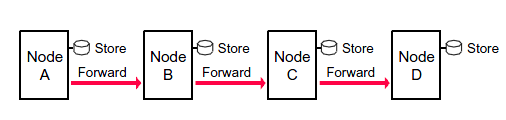
\includegraphics[scale=0.4]{store-and-forward.png}
\end{figure}
\end{center}
\end{frame}




\begin{frame}
\frametitle{Background: M2MShare}
\label{M2MShare}
%\textbf{M2MShare} aggiunge il sistema delle deleghe e lo utilizza all'interno di un protocollo Peer-to-peer per lo scambio di files fra dispositivi mobili.
\textbf{M2MShare} adotta alcune tecniche tipiche delle DTN per realizzare un applicazione Peer-to-Peer basata sulla prossimità fisica tra utenti, per lo scambio di files fra dispositivi mobili.
\ \\
\ \\
\pause 
Dispositivi dotati di:
\begin{itemize}
\item elevata mobilità
\item limitata autonomia energetica
\item limitato raggio di comunicazione
\item limitato spazio di storage
\end{itemize}
\end{frame}

\begin{frame}
\frametitle{Background: M2MShare}
L'elevata mobilità dei dispositivi costituirebbe un problema per dei protocolli tradizionali.\\
M2MShare utilizza tale mobilità, assieme ad un sistema di deleghe per ampliare l'area esplorata dai nodi interessati nella ricerca di un file.
\ \\

\pause
Elezione di nodi ``servant" e delega di tasks incompleti solo verso i nodi più promettenti: \\
\begin{center}
\textbf{nodi incontrati più frequentemente.}
\ \\
Esempio: 
\end{center}
\end{frame}


\begin{frame}
\label{Obiettivi}
\frametitle{Obiettivi della tesi}
\begin{itemize}
\item Implementare M2MShare in un ambiente di simulazione che permetta di valutarne l'efficienza considerando la mobilità dei nodi interessati
\item Confrontare l'efficienza di M2MShare rispetto altre strategie applicabili nello stesso contesto
\item Migliorare la versione esistente del protocollo aggiungendo la possibilità di delega multihop
\end{itemize}
\end{frame}


\begin{frame}
\label{ONE}
\frametitle{The ONE simulator}
\textbf{ONE}: \textbf{O}pportunistic \textbf{N}etwork \textbf{E}nvironment simulator.\\
Simulatore utilizzato per le nostre simulazioni.
\begin{itemize}
\item architettura modulare
\item diversi modelli di movimento disponibili
\item possibilità di emulare il comportamento di numerosi nodi in un ambiente realistico
\end{itemize}

\begin{figure}[ht]
\begin{minipage}[b]{0.4\linewidth}
\centering
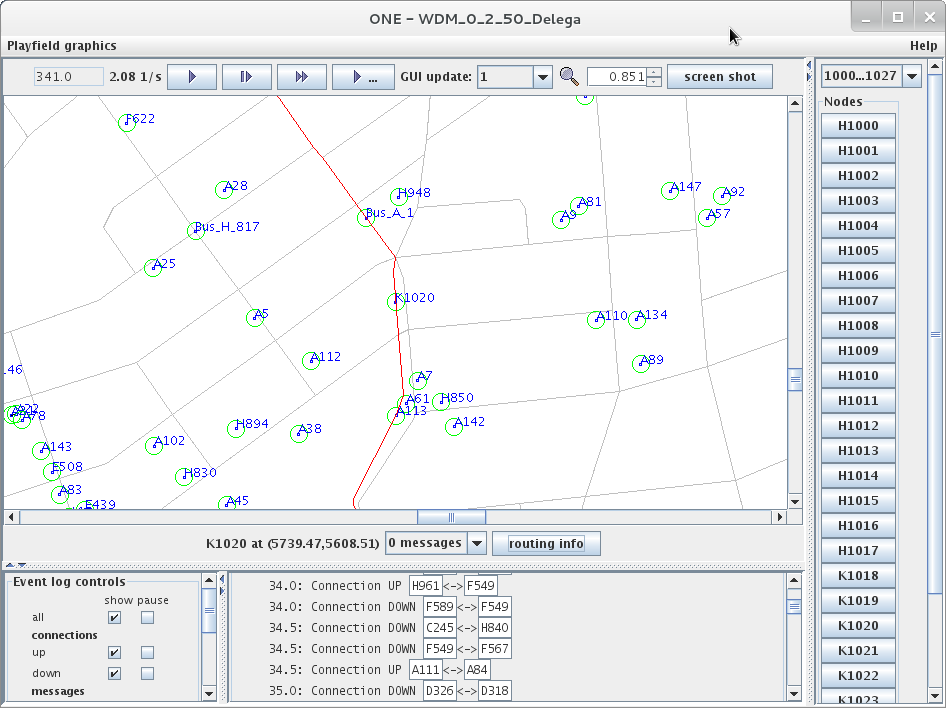
\includegraphics[scale=0.12]{img/Schermata-ONE.png}
\end{minipage}
\hspace{0.5cm}
\begin{minipage}[b]{0.4\linewidth}
\centering
%\pause
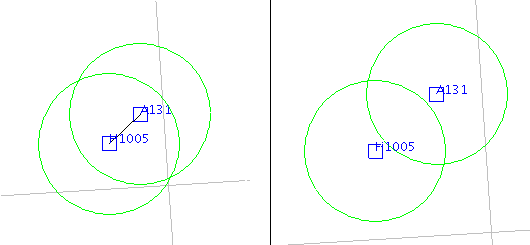
\includegraphics[scale=0.28]{img/connessioni.png}
\end{minipage}
\end{figure}
\end{frame}



\begin{frame}
\label{movement models}
\frametitle{Movement Models}
ONE consente di integrare nelle simulazioni diversi Movement Models.\\
\ \\
%\pause
Modelli analizzati durante il lavoro di tesi:
\begin{itemize}
\item Random Walk Movement
\item Random Waypoint Movement
%\pause
\item Random Map-Based Movement
\item Shortest Path Map-Based Movement
\item Routed Map-Based Movement
\item \textbf{Working Day Movement Model}
\end{itemize}
\end{frame}

\begin{frame}
\frametitle{Movement Models - WDM}
\label{WDM}
\textbf{Working Day Movement Model} (WDM)\\
simula la ripetitività delle azioni giornaliere svolte dalle persone durante i giorni lavorativi:
\ \\
\ \\
\begin{itemize}
\item dormire a casa
\item andare a lavoro in ufficio
\item uscire dopo il lavoro per shopping / serata con gli amici
\end{itemize}
\ \\
\ \\
\ \\
Descritto in: \\
{\footnotesize F. Ekman, A. Ker\"{a}nen, J. Karvo, J. Ott. ``Working day movement model", in Proc. of 1st ACM SIGMOBILE workshop, New York, NY, USA, 2008. }
\end{frame}

\begin{frame}
\frametitle{Movement Models - WDM}
WDM utilizza diversi sottomodelli per simulare diverse possibilità per i nodi di muoversi all'interno della mappa:
\ \\
\ \\
\begin{itemize}
\item camminando
\item guidando un mezzo proprio
\item utlizzare mezzi pubblici che si muovono secondo rotte prefissate
\end{itemize}
\end{frame}

\begin{frame}
\frametitle{La Mappa}
\label{mappa}
Mappa del centro cittadino di Helsinki:
\begin{figure}[htpb]

\begin{minipage}[b]{0.5\linewidth}
  \begin{center}
  	\multiinclude[format=png,graphics={scale=0.18}]{../figure/mappa/mappa}
%    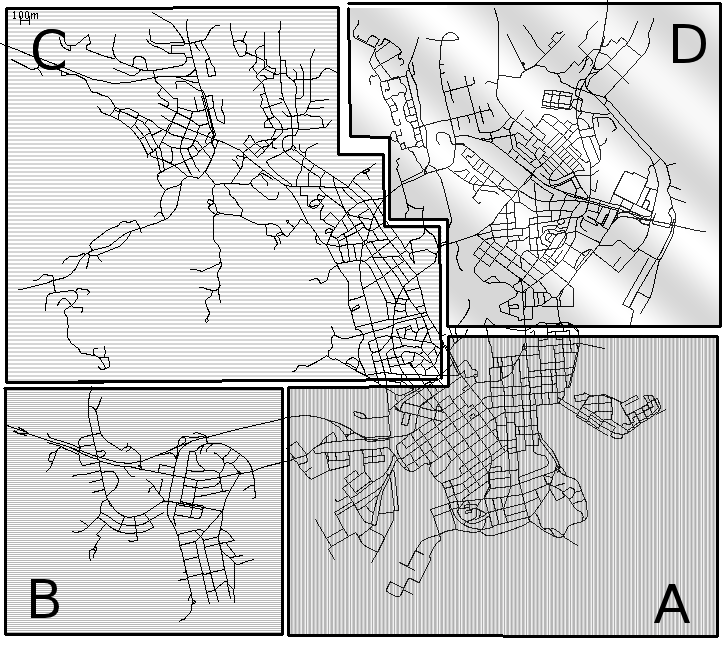
\includegraphics[scale=0.18]{../figure/mappa_ABCD.png}      
  \end{center}
\end{minipage}

\hspace{0.5cm}


\begin{minipage}[b]{0.5\linewidth}
\tiny 

\begin{center}
\begin{tabular}{|l|c|c|c|}
\hline
\textbf{District} & \textbf{Nodes} & \textbf{Offices} & \textbf{Meeting spots}\\
\hline
\hline
\bfseries A & 150 & 30 & 4 \\
\hline
\bfseries B & 50 & 10 & 1 \\
\hline
\bfseries C & 100 & 20 & 2 \\
\hline
\bfseries D & 100 & 20 & 2 \\
\hline
\bfseries E (A + B) & 100 & 20 & 2 \\
\hline
\bfseries F (A + C) & 150 & 30 & 4 \\
\hline
\bfseries G (A + D) & 150 & 30 & 4 \\
\hline
\bfseries H (Whole map) & 200 & 40 & 5 \\
\hline
\end{tabular}
\end{center}   
\label{tabellaDistrettiMappa}

\normalsize
\end{minipage}

\end{figure}
\end{frame}
%
%\begin{frame}
%\frametitle{Simulazioni}
%Obiettivo: analizzare l'efficienza di M2MShare in termini di tempo di recupero del file cercato rispetto ad altre due strategie, una che non utilizza deleghe, l'altra in cui si delegano task indiscriminatamente a tutti i nodi incontrati.
%\small
%\begin{table}[h]
%\begin{center}
%\begin{tabular}{|l|r|}
%\hline
%\bfseries Population & 1000 \\
%\hline
%\bfseries File size & 3.0 MB \\
%\hline
%\bfseries File popularity & 50 copies uniformly chosen \\
%\hline
%\bfseries Delegation type & No\_delegation, M2MShare, Delegation\_to\_all \\
%\hline
%\bfseries Delegation depth & 1 \\
%\hline
%\bfseries File Division Strategy & M2MShare \\
%\hline
%\bfseries Nr. of simulations & 40 x 3\\
%\hline
%\bfseries Simulated time & One week \\
%\hline
%\end{tabular}
%\end{center}
%\end{table}
%\normalsize
%\end{frame}
%
%\begin{frame}
%\frametitle{Simulazioni}
%Obiettivo: analizzare l'efficienza di M2MShare rispetto alle altre due strategie, con diversi valori di popolarità del file cercato.
%\small
%\begin{table}[h]
%\begin{center}
%\begin{tabular}{|l|r|}
%\hline
%\bfseries Population & 1000 \\
%\hline
%\bfseries File size & 3.0 MB \\
%\hline
%\bfseries File popularity & 50, 100, 150, 200, 250, 300, 350, 400 copies \\
%\hline
%\bfseries Delegation type & No\_delegation, M2MShare, Delegation\_to\_all \\
%\hline
%\bfseries Delegation depth & 1 \\
%\hline
%\bfseries File Division Strategy & M2MShare \\
%\hline
%\bfseries Nr. of simulations & 40 x 8 x 3\\
%\hline
%\bfseries Simulated time & 48 hours \\
%\hline
%\end{tabular}
%\end{center}
%\end{table}
%\normalsize
%\end{frame}
%
%\begin{frame}
%\frametitle{Simulazioni}
%Obiettivo: analizzare l'efficienza di M2MShare rispetto alle altre due strategie, con diversi valori di popolazione totale nel mondo simulato.
%\small
%\begin{table}[h]
%\begin{center}
%\begin{tabular}{|l|r|}
%\hline
%\bfseries Population & 100, 200, 400, 600, 800, 1000 \\
%\hline
%\bfseries File size & 3.0 MB \\
%\hline
%\bfseries File popularity & 5\%, 10\%, 50\% \\
%\hline
%\bfseries Delegation type & No\_delegation, M2MShare, Delegation\_to\_all \\
%\hline
%\bfseries Delegation depth & 1 \\
%\hline
%\bfseries File Division Strategy & M2MShare \\
%\hline
%\bfseries Nr. of simulations & 40 x 6 x 3 x 3\\
%\hline
%\bfseries Simulated time & 48 hours \\
%\hline
%\end{tabular}
%\end{center}
%\end{table}
%\normalsize
%\end{frame}
%
%\begin{frame}
%\frametitle{Simulazioni}
%Obiettivo: analizzare l'efficienza di M2MShare originale (1-hop delegations) rispetto alla nostra versione aggiornata (con deleghe fino a 3 hop)
%\small
%\begin{table}[h]
%\begin{center}
%\begin{tabular}{|l|r|}
%\hline
%\bfseries Population & 1000 \\
%\hline
%\bfseries File size & 3.0 MB \\
%\hline
%\bfseries File popularity & 25 copies in a single district \\
%\hline
%\bfseries Delegation type & No\_Delegation, M2MShare\\
%\hline
%\bfseries Delegation depth & 1, 3 \\
%\hline
%\bfseries File Division Strategy & M2MShare \\
%\hline
%\bfseries Nr. of simulations & 40 x 3\\
%\hline
%\bfseries Simulated time & One week \\
%\hline
%\end{tabular}
%\end{center}
%\end{table}
%\normalsize
%\end{frame}
%
%\begin{frame}
%\frametitle{Simulazioni}
%Obiettivo: analizzare l'efficienza di M2MShare in termini di ridondanza totale di dati generata all'interno della rete.
%\small
%\begin{table}[h]
%\begin{center}
%\begin{tabular}{|l|r|}
%\hline
%\bfseries Population & 1000 \\
%\hline
%\bfseries File size & 3.0 MB \\
%\hline
%\bfseries File popularity & 50 copies uniformly chosen \\
%\hline
%\bfseries Delegation type & M2MShare, Delegation\_to\_all \\
%\hline
%\bfseries Delegation depth & 1 \\
%\hline
%\bfseries File Division Strategy & M2MShare \\
%\hline
%\bfseries Nr. of simulations & 40 x 2\\
%\hline
%\bfseries Simulated time & One week \\
%\hline
%\end{tabular}
%\end{center}
%\end{table}
%\normalsize
%\end{frame}
%
%\begin{frame}
%\frametitle{Simulazioni}
%Obiettivo: analizzare l'efficienza della File Division Strategy di M2MShare rispetto ad altre due tecniche, una in cui ogni trasferimento di file comincia dall'inizio del file, l'altra in cui il punto iniziale del trasferimento viene scelto casualmente per ogni trasferimento.
%\small
%\begin{table}[h]
%\begin{center}
%\begin{tabular}{|l|r|}
%\hline
%\bfseries Population & 1000 \\
%\hline
%\bfseries File size & 3.0 MB, 10.0 MB, 25.0 MB \\
%\hline
%\bfseries File popularity & 50 copies uniformly chosen \\
%\hline
%\bfseries Delegation type & M2MShare \\
%\hline
%\bfseries Delegation depth & 1 \\
%\hline
%\bfseries File Division Strategy & M2MShare, iM , rM \\
%\hline
%\bfseries Nr. of simulations & 40 x 3 x 3\\
%\hline
%\bfseries Simulated time & One week \\
%\hline
%\end{tabular}
%\end{center}
%\end{table}
%\normalsize
%\end{frame}

\begin{frame}
\label{Esperimenti}
\frametitle{Esperimenti}
\textbf{Obiettivo:} analizzare l'efficienza di M2MShare in termini di tempo di recupero del file cercato rispetto ad altre due strategie, una che non utilizza deleghe, l'altra in cui si delegano task indiscriminatamente a tutti i nodi incontrati.\\
\ \\
%\pause
Metriche analizzate:
\begin{itemize}
\item Tempo di reperimento
\item Numero di deleghe utilizzate
\item Percentuale di task completati con successo
\item Ridondanza introdotta nella rete
\end{itemize}
\end{frame}

\begin{frame}
\frametitle{Risultati}
\begin{center}
\begin{figure}[ht]
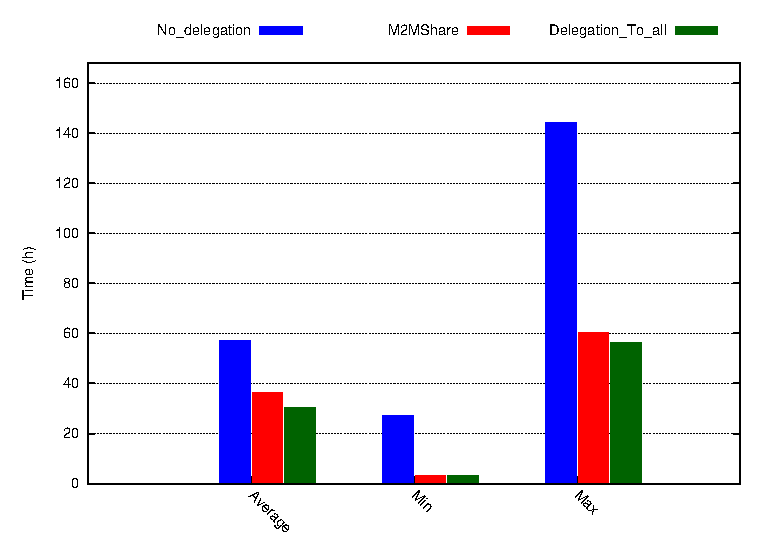
\includegraphics[scale=0.7]{tempi.eps}
\caption{Average, min and max time employed by each strategy to find the required data file}
\end{figure}
\end{center}
\end{frame}

\begin{frame}
\frametitle{Risultati}
\begin{figure}[ht]
\begin{minipage}[b]{0.45\linewidth}
\centering
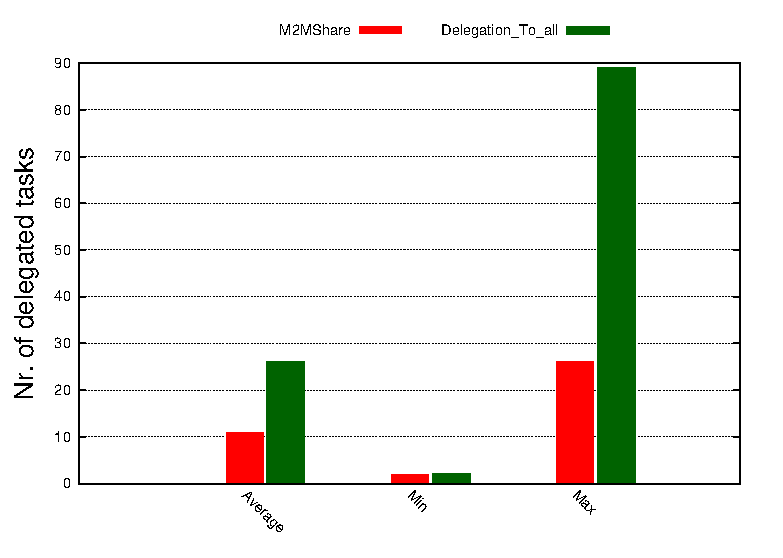
\includegraphics[scale=0.4]{delegheFatte.eps}
\caption{Average, min, max number of delegations employed by each delegation strategy}
\end{minipage}
\hspace{0.5cm}
\begin{minipage}[b]{0.45\linewidth}
\centering
%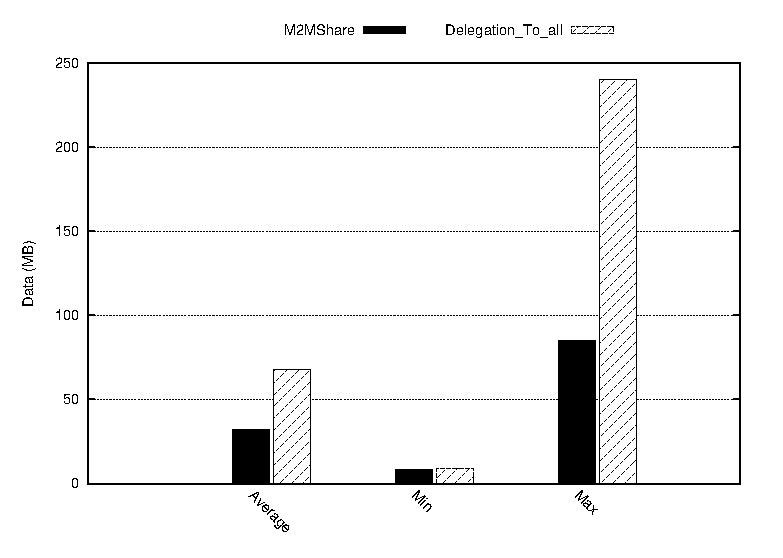
\includegraphics[scale=0.4]{../grafici/data.eps}
%\caption{Average, min, max number of delegations employed by each delegation strategy}
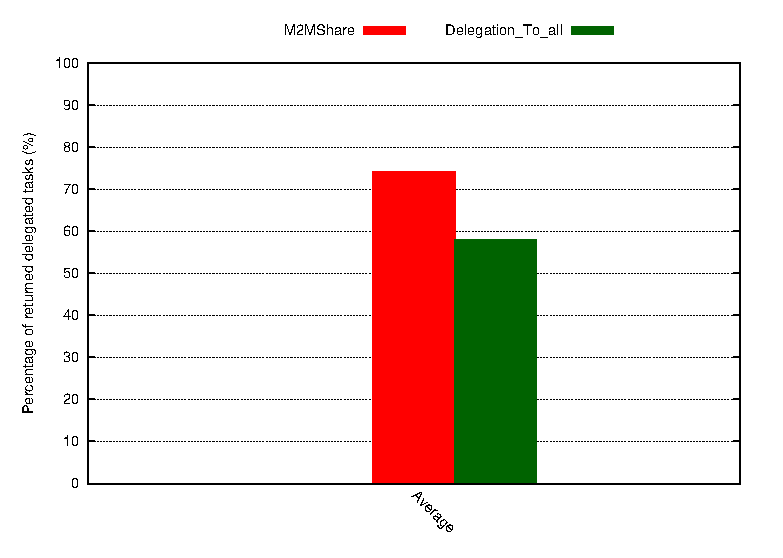
\includegraphics[scale=0.4]{percDeleghe.eps}
\caption{Percentage of completed tasks against the number of overall delegations employed}
\end{minipage}
\end{figure}
\end{frame}


%\begin{frame}
%\frametitle{Risultati}
%\begin{figure}[ht]
%\begin{minipage}[b]{0.4\linewidth}
%\centering
%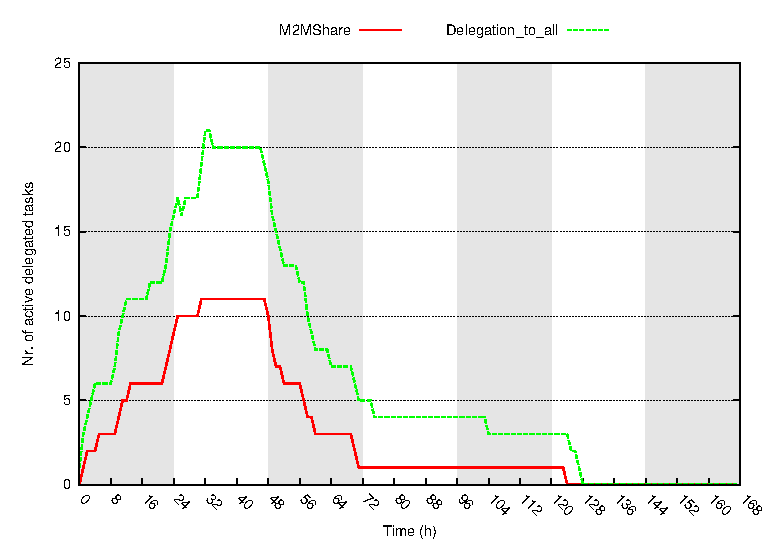
\includegraphics[scale=0.4]{../grafici/delegheAttive.eps}
%%\caption{Average number of simultaneously active delegated tasks}
%\end{minipage}
%
%%\hspace{0.5cm}
%
%%\begin{minipage}[b]{0.40\linewidth}
%%\centering
%%\pause
%%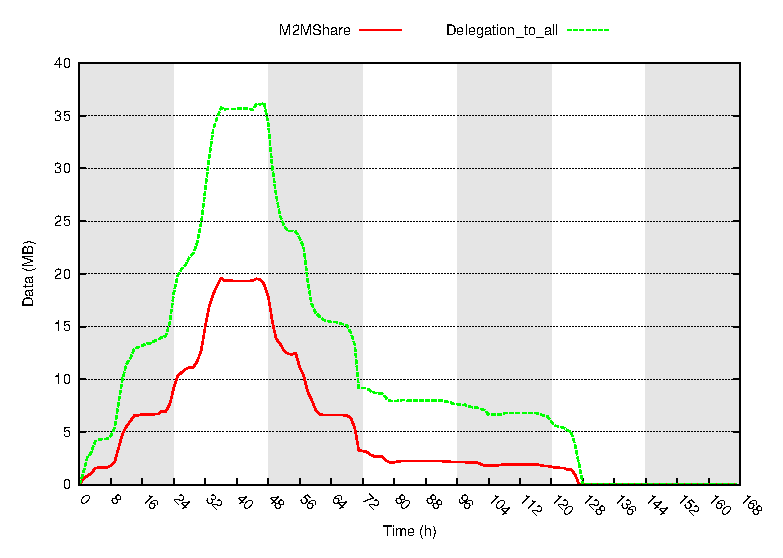
\includegraphics[scale=0.3]{../grafici/ridondanza.eps}
%%\caption{Average data redundancy in the network}
%%\end{minipage}
%
%\begin{minipage}[b]{0.4\linewidth}
%\centering
%\pause
%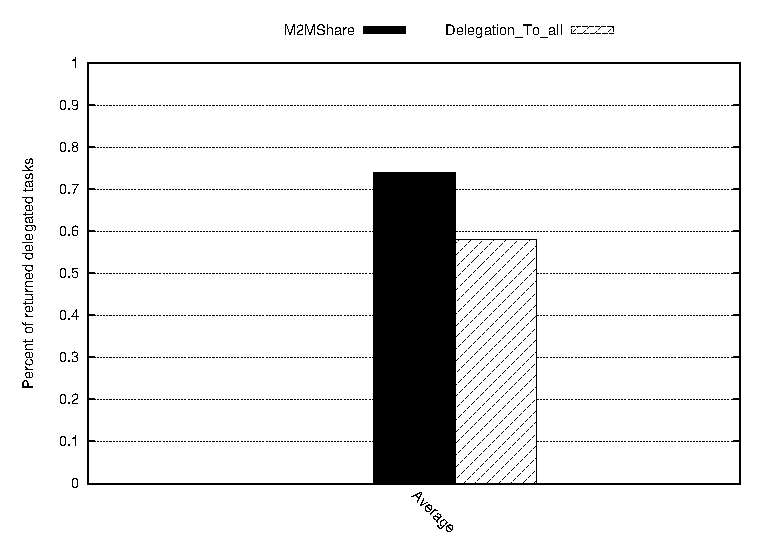
\includegraphics[scale=0.4]{../grafici/percDeleghe.eps}
%%\caption{Percentage of completed previously delegated tasks against the number of overall delegations employed.}
%\end{minipage}
%
%\end{figure}
%\end{frame}
%
%
%\begin{frame}
%\frametitle{Risultati}
%\begin{center}
%\begin{figure}[ht]
%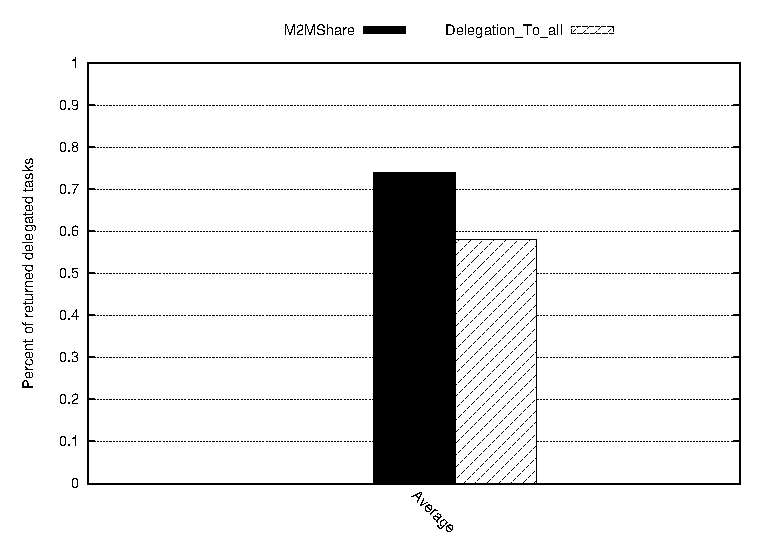
\includegraphics[scale=0.7]{../grafici/percDeleghe.eps}
%\caption{Percentage of completed previously delegated tasks against the number of overall delegations employed.}
%\end{figure}
%\end{center}
%\end{frame}

\begin{frame}
\label{diversa pop}
\frametitle{Risultati}
\begin{center}
\begin{figure}[ht]
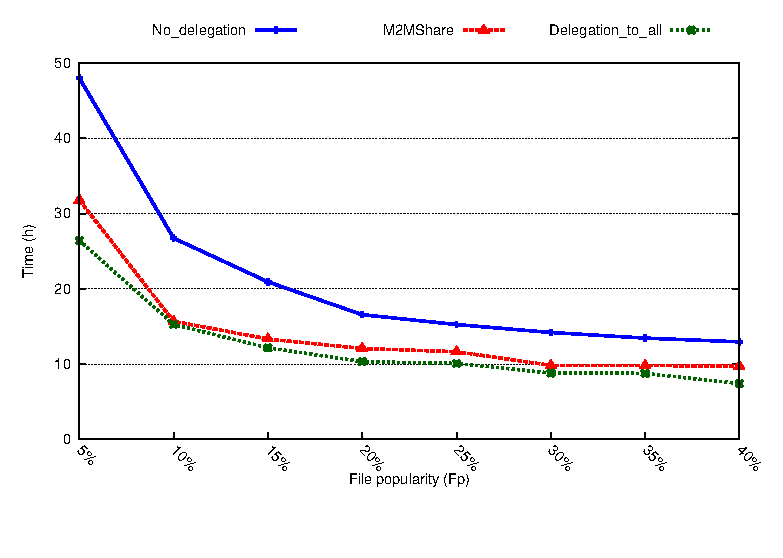
\includegraphics[scale=0.7]{tempiVFDiversaPop_zoom.eps}
    \caption{Average retrieval time with variable file popularity}
\end{figure}
\end{center}
\end{frame}
%
%\begin{frame}
%\frametitle{Risultati}
%\begin{center}
%\begin{figure}[ht]
%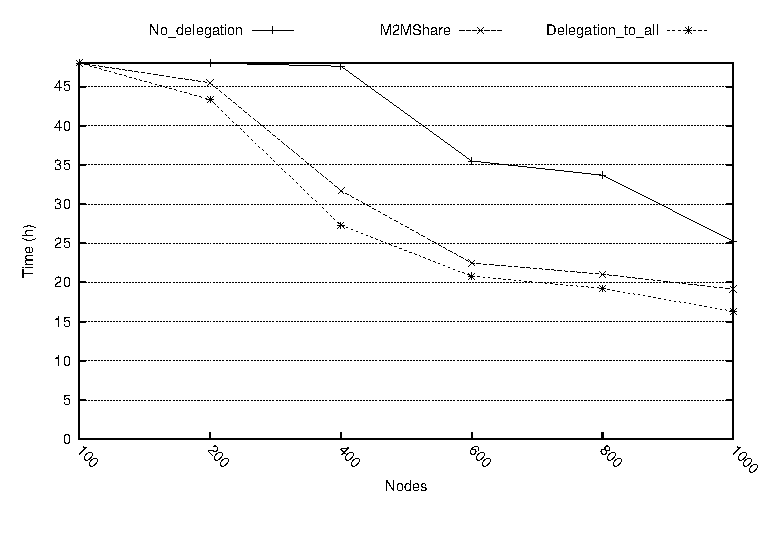
\includegraphics[scale=0.7]{../grafici/tempiVF_Fp5.eps}
%\caption{Average found time with $Fp = 5\%$}
%\end{figure}
%\end{center}
%\end{frame}
%
%\begin{frame}
%\frametitle{Risultati}
%\begin{center}
%\begin{figure}[ht]
%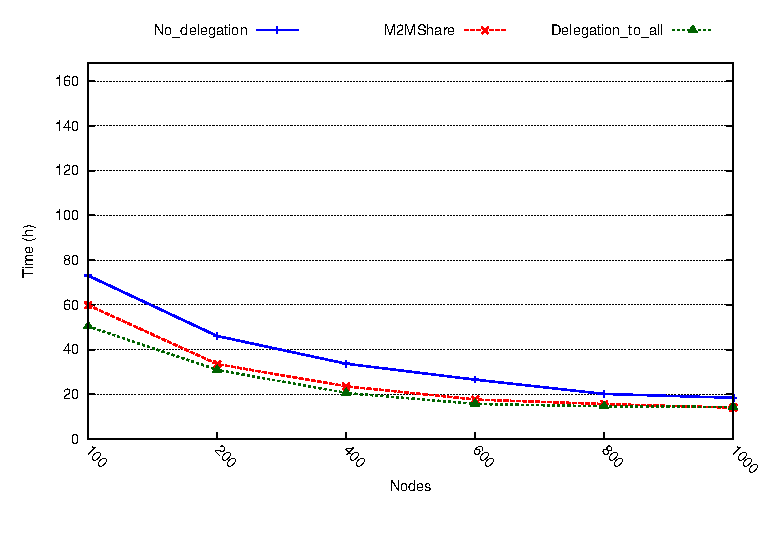
\includegraphics[scale=0.7]{../grafici/tempiVF_Fp10.eps}
%\caption{Average found time with $Fp = 10\%$}
%\end{figure}
%\end{center}
%\end{frame}
%
%\begin{frame}
%\frametitle{Risultati}
%\begin{center}
%\begin{figure}[ht]
%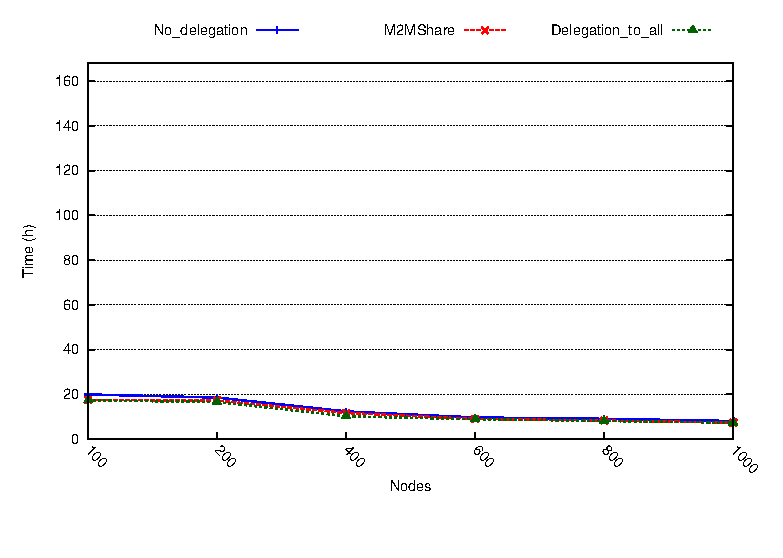
\includegraphics[scale=0.7]{../grafici/tempiVF_Fp50.eps}
%\caption{Average found time with $Fp = 50\%$}
%\end{figure}
%\end{center}
%\end{frame}

\begin{frame}
\frametitle{Esperimenti}
\label{descrizione multi hop}
\textbf{Obiettivo:} aggiornare M2MShare aggiungendo la possibilità di delega multi-hop per estendere efficientemente il raggio di azione ed analizzare l’efficienza di M2MShare originale (1-hop) rispetto alla nuova versione  (con deleghe fino a 3 hop)
\end{frame}

\begin{frame}
\frametitle{Risultati}
\label{mappa multi hop}
\begin{figure}[htbp]
\centering%
\vspace{-30pt}%
\setcounter{subfigure}{0}%
\subfigure[Explored area with {1-hop}]%
{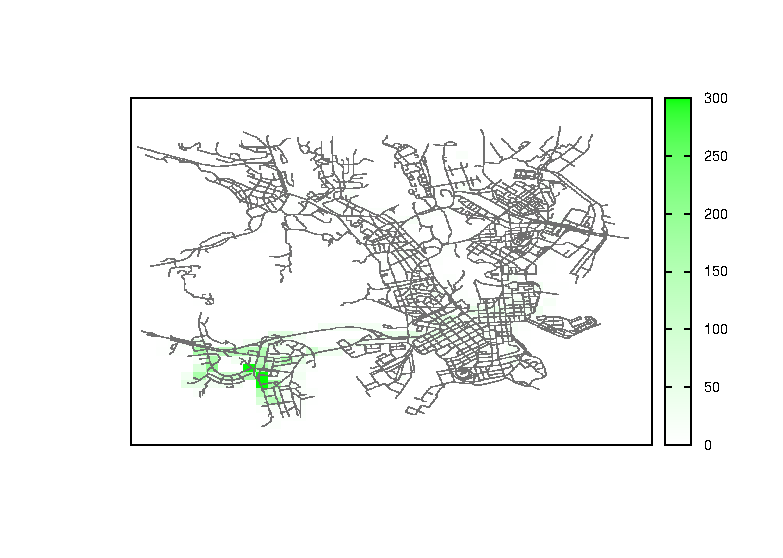
\includegraphics[scale=0.38]{../grafici/mappe/M2MShare_1_hop_50perc.eps}}\qquad
\vspace{-10pt}%
\pause
\subfigure[Explored area with 2-hop]%
{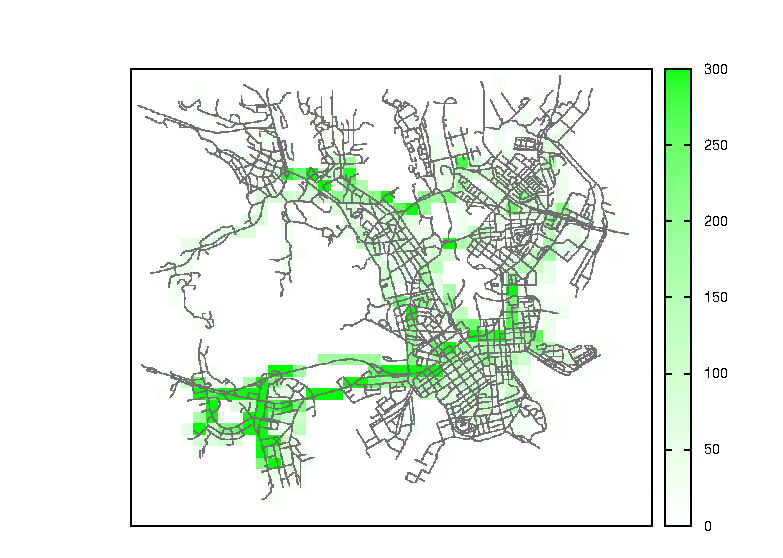
\includegraphics[scale=0.38]{../grafici/mappe/M2MShare_2_hop_50perc.eps}}\qquad
\vspace{-10pt}%
\pause
\subfigure[Explored area with 3-hop]%
{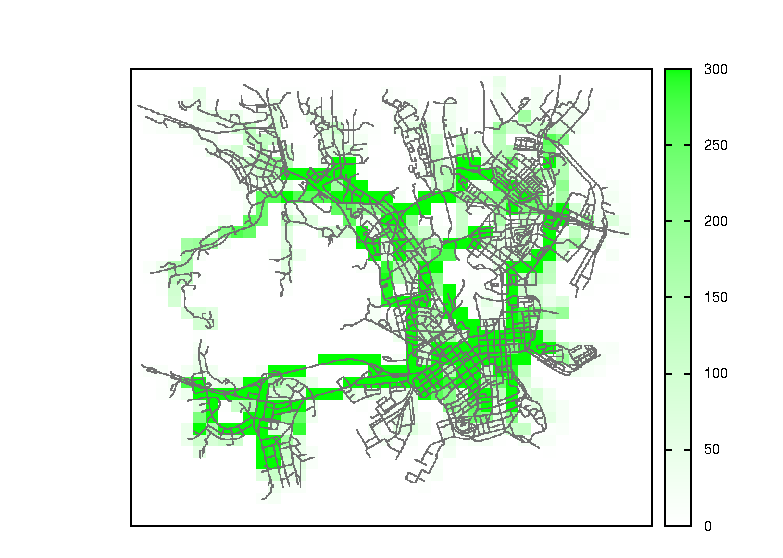
\includegraphics[scale=0.38]{../grafici/mappe/M2MShare_3_hop_50perc.eps}}
\end{figure}
\end{frame}


\begin{frame}
\frametitle{Risultati}
\begin{center}
\begin{figure}[ht]
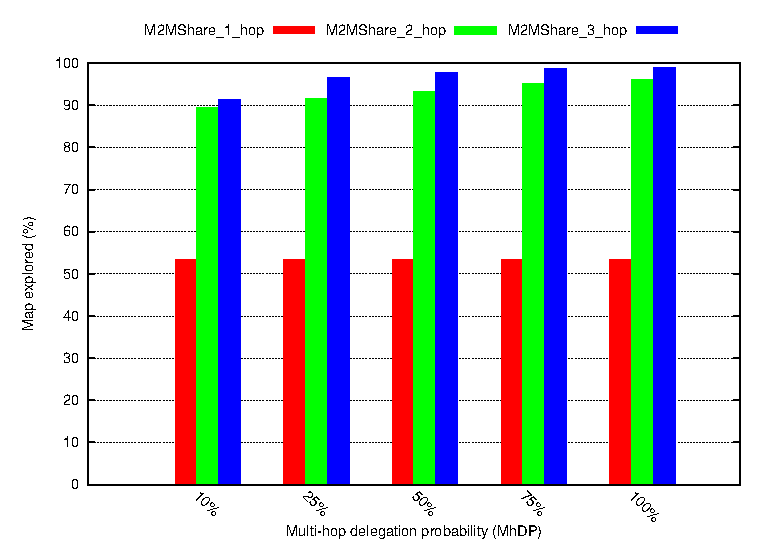
\includegraphics[scale=0.7]{mapCovered_MultiHop.eps}
\caption{Average percentage of explored area employing M2MShare with different multi-hop versions}
\end{figure}
\end{center}
\end{frame}

\begin{frame}
\frametitle{Risultati}
\begin{center}
\begin{figure}[ht]
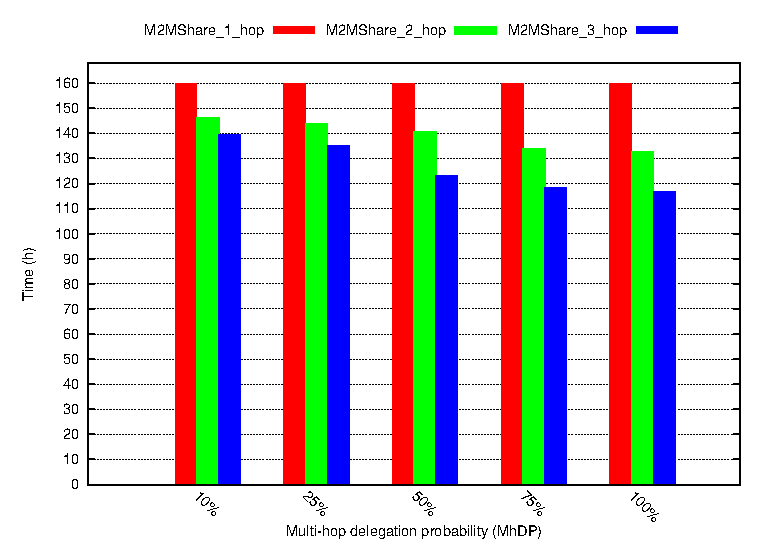
\includegraphics[scale=0.7]{tempiVF_MultiHop.eps}
\caption{Average found time employed by M2MShare with different multi-hop versions in finding the required data file}
\end{figure}
\end{center}
\end{frame}


\begin{frame}
\frametitle{Risultati}
Il sistema di deleghe multi-hop aumenta il numero di nodi interessati, con conseguente aumento della ridondanza
\begin{center}
\begin{figure}[ht]
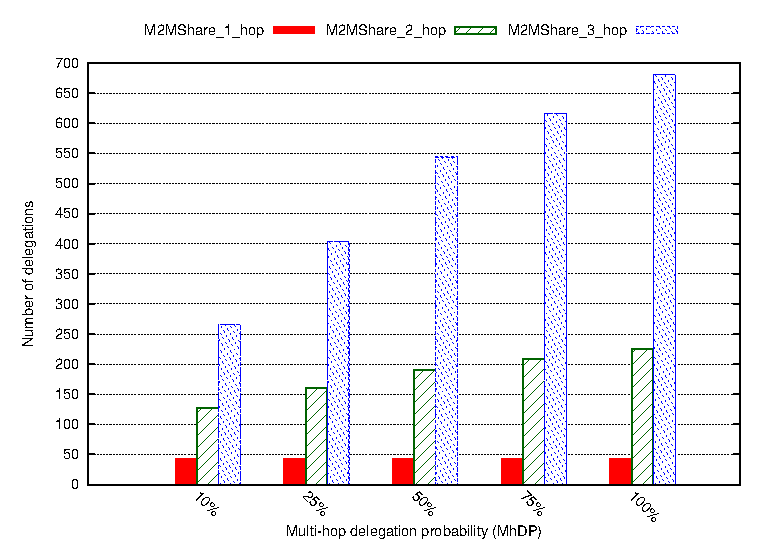
\includegraphics[scale=0.55]{delegheMultiHopPerc.eps}
\caption{Avg. delegations used, M2MShare with different multi-hop versions}
\end{figure}
\end{center}
\end{frame}




%\begin{frame}
%\frametitle{Risultati}
%\begin{center}
%\begin{figure}[ht]
%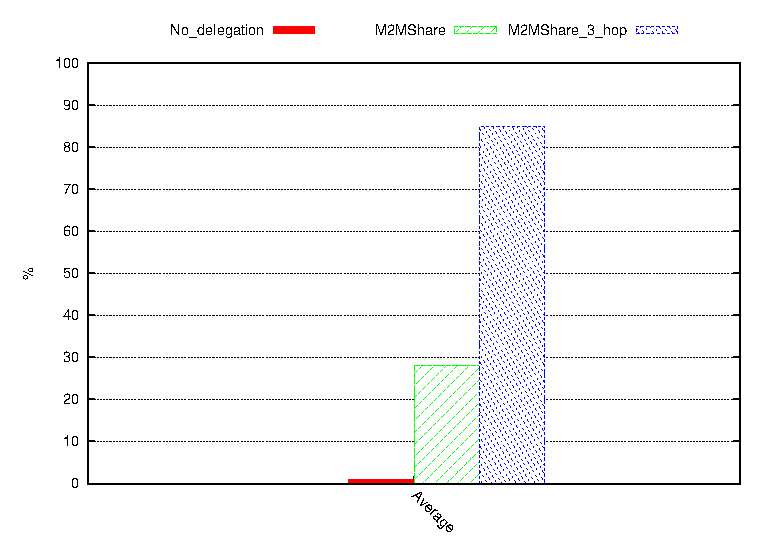
\includegraphics[scale=0.7]{../grafici/percCompletaMultiHop.eps}
%\caption{Percentage of successfully completed simulations with searched file far from requester}
%\end{figure}
%\end{center}
%\end{frame}
%
%\begin{frame}
%\frametitle{Risultati}
%\begin{center}
%\begin{figure}[ht]
%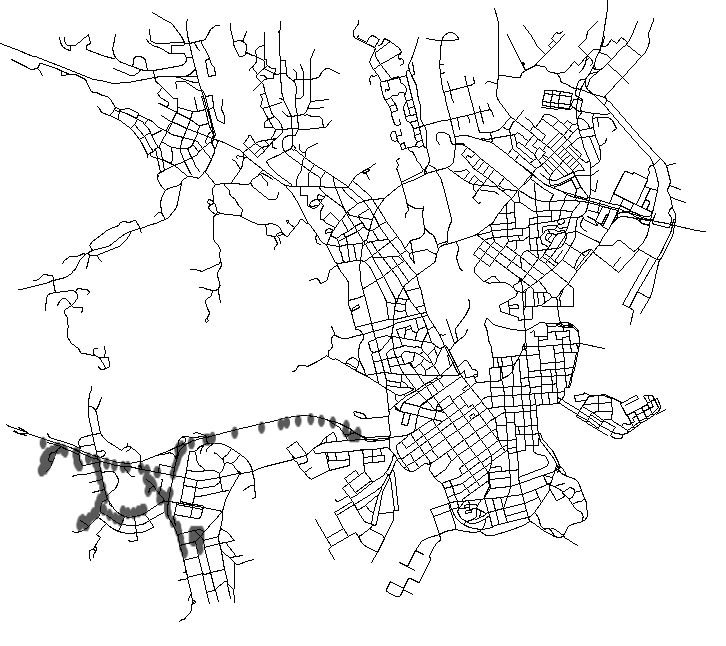
\includegraphics[scale=0.25]{../figure/mappa_0_hop.png}
%    \caption{Explored area without use of delegations}
%\end{figure}
%\end{center}
%\end{frame}
%
%\begin{frame}
%\frametitle{Risultati}
%\begin{center}
%\begin{figure}[ht]
%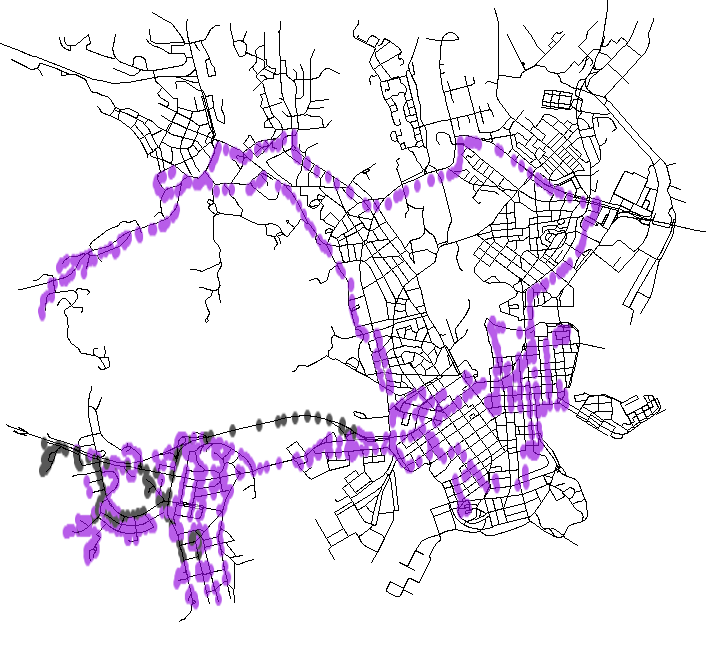
\includegraphics[scale=0.25]{../figure/mappa_1_hop.png}
%    \caption{Explored area using M2MShare and 1-hop delegations}
%\end{figure}
%\end{center}
%\end{frame}
%
%\begin{frame}
%\frametitle{Risultati}
%\begin{center}
%\begin{figure}[ht]
%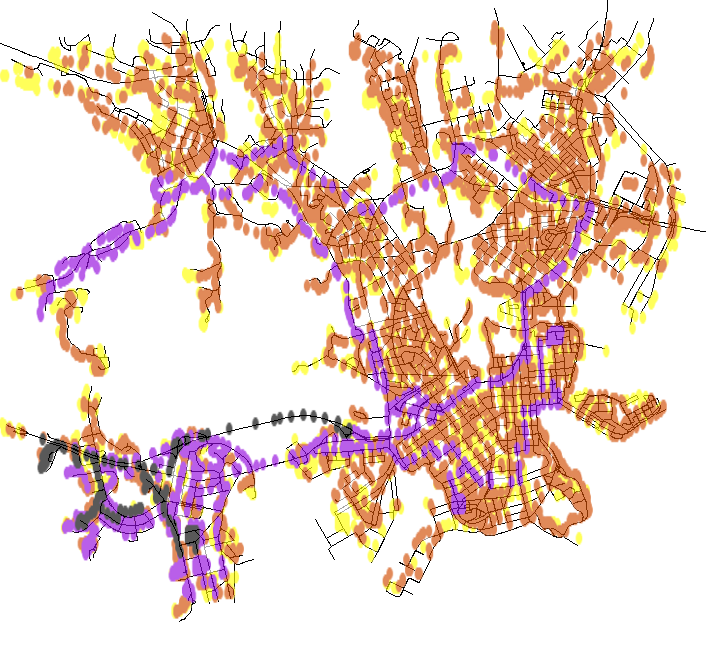
\includegraphics[scale=0.25]{../figure/mappa_3_hop.png}
%    \caption{Explored area using M2MShare and up to 3-hop delegations}
%\end{figure}
%\end{center}
%\end{frame}
%
%\begin{frame}
%\frametitle{Risultati}
%\begin{center}
%\begin{figure}[ht]
%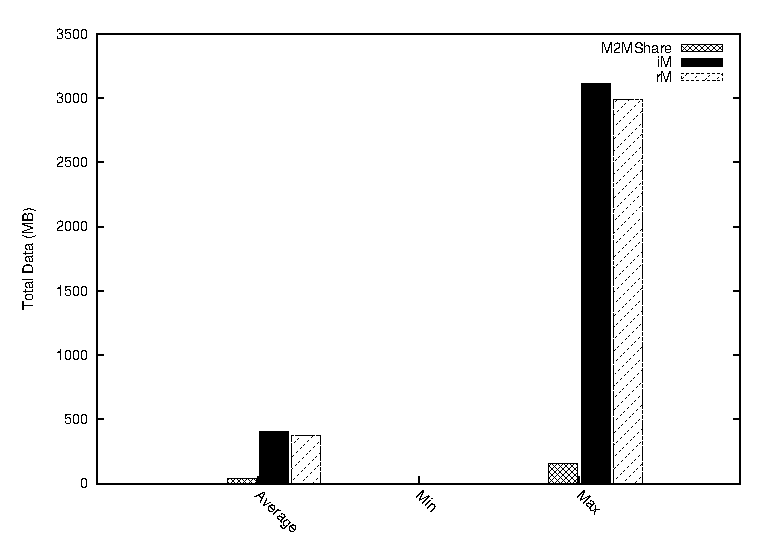
\includegraphics[scale=0.7]{../grafici/dataDFS_3MB.eps}
%\caption{Average, min, max transferred data amount using different file division strategies and 3.0 MB file size.}
%\end{figure}
%\end{center}
%\end{frame}
%
%\begin{frame}
%\frametitle{Risultati}
%\begin{center}
%\begin{figure}[ht]
%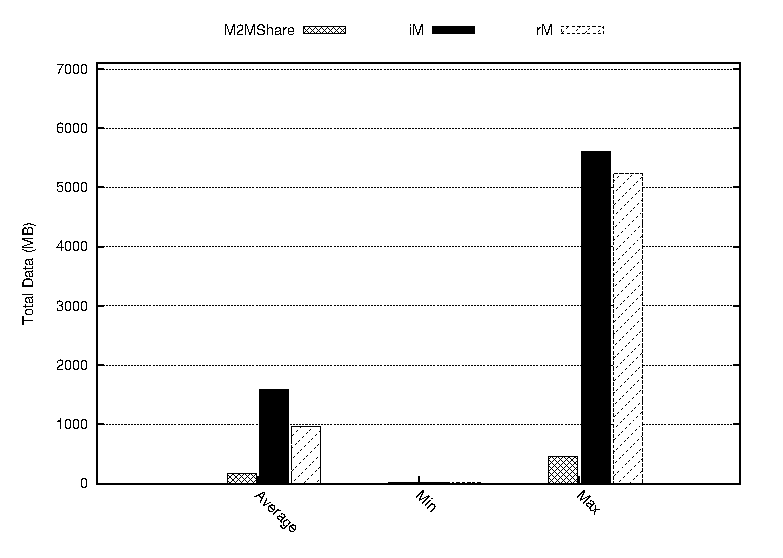
\includegraphics[scale=0.7]{../grafici/dataDFS_10MB.eps}
%\caption{Average, min, max transferred data amount using different file division strategies and 10.0 MB file size.}
%\end{figure}
%\end{center}
%\end{frame}
%
%\begin{frame}
%\frametitle{Risultati}
%\begin{center}
%\begin{figure}[ht]
%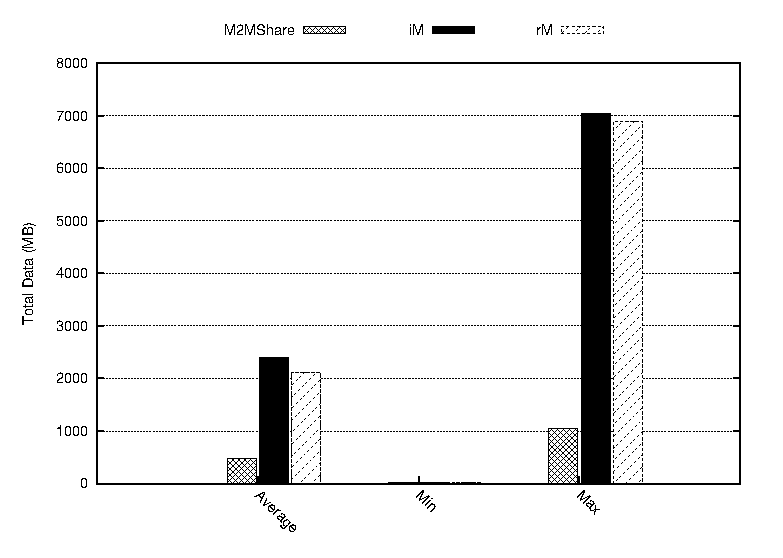
\includegraphics[scale=0.7]{../grafici/dataDFS_25MB.eps}
%\caption{Average, min, max transferred data amount using different file division strategies and 25.0 MB file size.}
%\end{figure}
%\end{center}
%\end{frame}

\begin{frame}
\frametitle{Riassumendo}
\label{Riassumendo}
\begin{itemize}
\item Implementato M2MShare in un ambiente di simulazione realistico, che ci ha permesso di valutarne l'efficienza considerando la mobilità dei nodi interessati
%\pause
\item Verificato l'efficienza di M2MShare rispetto altre strategie applicabili nello stesso contesto
%\pause
\item Migliorato il protocollo esistente aggiungendo la possibilità di delega a più hops
%\pause
\item Migliorato il simulatore ONE aggiungendo delle features condivise con la comunità di utenti
%\pause
\item Risultati preliminari pubblicati su\\
A. Bujari, C. E. Palazzi, D. Bonaldo, ``Performance Evaluation of a File Sharing DTN Protocol with Realistic Mobility", in Proc. of IFIP/IEEE Wireless Days 2011, Niagara
Falls, Ontario, Canada, Oct 2011
%Wireless Days Conference 2011 (\href{http://www.wireless-days.org/}{http://www.wireless-days.org}) in Niagara Falls, Ontario, Canada.
\end{itemize}
\end{frame}

\begin{frame}
\frametitle{\ }
\begin{center}
Grazie per l'attenzione.
\end{center}
\end{frame}



\end{document}